\chapter{Tk\stochsim{}: user guide}

The original \stochsim{} simulator was written for Microsoft Windows and was
provided with a graphical user interface (GUI) based on the Microsoft MFC
widgets.  Although the core simulation engine was written an ANSI C++, and
therefore could be ported to other operating systems with relative ease, the
widgets used for the GUI were not compatible with other operating systems such
as UNIX, Linux, or MacOS.  Therefore to run \stochsim{} under such operating
systems, the user was required to write the simulation initialisation files
manually. This is tedious and error-prone. In order to ease the creation and
modification of simulation configurations under a larger number of operating
environments, a novel interface written in Perl using the Tk widgets was
developed. This interface has been written and tested under Debian/GNU Linux,
but should run under most modern operating systems for which a Perl/Tk exists
(It has also been tested under Microsoft Windows98). The current interface
requires at least Perl 5.005 and Perl/Tk 800.022. 

\parpic[r]{\scalebox{0.4}{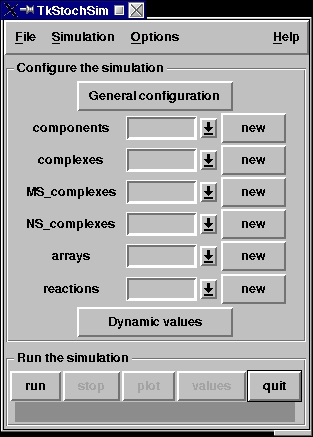
\includegraphics{main.jpg}}} When Tk\stochsim{} is
launched, the main window appears on the screen.  Tk\stochsim{} can be
controlled with either the mouse or the keyboard.  When using the keyboard,
pressing the <tab> key allows you to switch the focus between the various
widgets (buttons, text boxes, etc.) of the interface.  A focused widget can be
activated by pressing the <space> bar or the <return> key. The menus can also be
activated via the keyboard by the sequences \mbox{<Alt-f>} (``File'' menu),
\mbox{<Alt-s>} (``Simulation'' menu), \mbox{<Alt-o>} (``Option'' menu) and
\mbox{<Alt-h>} (``Help'' menu). You can quit the program by clicking on the
``quit'' button or pressing \mbox{<Ctrl-q>}.

The ``File'' menu is used to open an existing simulation (accelerator:
\mbox{<Ctrl-o>}), to save the current configuration (accelerator:
\mbox{<Ctrl-s>}), to create a new simulation or to rename the current simulation
(accelerator: \mbox{<Ctrl-a>}) or to quit (accelerator: \mbox{<Ctrl-q>}). You
can also import or export simple simulations using the SBML language
level1\footnote{See
  \url{http://www.cds.caltech.edu/erato/sbml/docs/index.html}.}  designed by the
\textsc{erato} project on systems biology.  The ``File'' menu also presents a
history of past simulations, providing an easy and fast access to them.
  
The ``Simulation'' menu currently presents only two options, one to run a
simulation (accelerator: \mbox{<Ctrl-r>}) and one to stop the simulation
(accelerator: \mbox{<Ctrl-w>}). This last option is currently not activated
under Microsoft Windows.

The ``Options'' menu permits to configure the interface and to activate or
deactivate the helping balloons on the fly (accelerators: \mbox{<Ctrl-b>} and
\mbox{<Ctrl-n>} respectively).  Those balloons present a short explanation on
the use of the different items of the interface. It is a good idea to explore
the graphical interface at least once with the balloons activated. You can
systematically desactivate the balloons by setting the ``balloon'' option to off
in the file \texttt{stochsimrc}.  This file is present in the directory ``lib''
of the distribution. It contains information about the setup of the Perl/Tk
interface.  A copy of this file is normally installed in the personal directory
\texttt{.stochsim} of each user (or in the directory \texttt{config\_examples}
under Microsoft Windows9x). The configuration of the interface can be partially
done through the \emph{Preferences} window (accelerator: \mbox{<Ctrl-P>}).  All
the changes will be recorded in \texttt{stochsimrc} when the program will quit.
The file can also be manually edited with any text editor.

Finally, the ``help'' menu provides the legal informations about the programs
and access to a PDF version of the present manual. The
first time you'll ask for the PDF version, the program shall ask you to point
the location of your favourite PDF reader. It will normally remind it afterward.
The address is kept by the option ``pdfreader'' in the file \texttt{stochsimrc}.

All the accelerators described should be directly available from the main
window, without the need to open the menus.

\section{Opening and saving a simulation}

All the simulations should normally be stored in a specific directory (although
this is not an obligation). Under Unix-like systems, this
directory is \texttt{\$HOME/.stochsim}. Under Microsoft Windows9x the
simulations are stored in the subdirectory \texttt{config\_examples} of the
\stochsim{} distribution.  Each simulation is stored in a subdirectory, the
name of which is specified by the user. The structure of this directory is
constant.  It contains two subdirectories, \texttt{Input} and \texttt{Output},
containing the \texttt{*.INI} and \texttt{*.OUT} files respectively.

To open an existing simulation, you can go to the menu-bar and select
``File->Open...'', or type \mbox{<Ctrl-o>}. Then select an existing simulation
configuration file (usually named \texttt{STCHSTC.INI}). The usage of the file
selector could be lightly different according to the running operating system.
However, since it is the usual file selector of your windows manager, its
description is out of the scope of the present manual. Tk\stochsim{} will
remind the last directory visited to look for a simulation. It is stored by the
option ``confdir'' in the file \texttt{stochsimrc}. You can also setup the
default directory with the \emph{Preferences} window.

To save a configuration under its previous name, you can go to the menu-bar and
select ``File->Save'' or type \mbox{<Ctrl-s>}. Note that the current configuration
is automatically saved when a simulation is launched.

To create a new configuration or to save the current configuration under a
different name, you can to the menu-bar and select ``File->Save as...'' or type
\mbox{<Ctrl-a>}, and then select an existing \texttt{STCHSTC.INI} (in the
subdirectory \texttt{Input} of an existing simulation) or type the name of the
new \emph{main} directory.


\section{Setting up a simulation}

\subsection{General configuration}\label{genconfig}

\parpic{\scalebox{0.4}{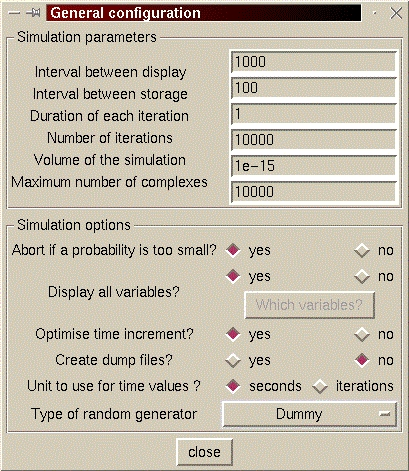
\includegraphics{mainconf.jpg}}} To create a new
simulation, you need to setup a general configuration first. To do so, click on
the button labelled ``General configuration''.  
% previous has to be located before the screenshot, but put here for easthetics
The \emph{General configuration} window is then opened, where you can modify
several options of the simulation.  The detailled explanation of the various
options is given in the chapter \ref{conf_files}. 

The ``interval between storage'' controls the frequency of the variable
recording, and hence the data shown in the graphical display (see section
\ref{display}). There is a relationship between the ``duration of the
simulation'' and the ``interval between storage''. You could be ask to change
the latter by \stochsim.

The option ``duration of each iteration'' is meaningfull only if you do not
allow the optimisation of the time increment. In such a case, you will have to
set-up the time increment by trial error. Indeed, if the time increment is too
small, the probability that no reaction takes place during an iteration becomes
significant and the simulation is inefficient. On the contrary, if the time
increment is too big, several reactions should take place during one iteration,
which cannot be the case with \stochsim{}. 

The limit for the ``maximal number of complexes'' is \MAXLIMITCOMPLEXES. This
value is far higher than what we can expect to use in a \stochsim{} simulation
anyway (except if you are ready to wait the results for twenty years). Be sure
to check the option ``use spatial extensions'' if you want to use the
bidimensional lattices implemented since \stochsim{} 1.2.

You'd rather not touch most of the options in the frame ``Simulation options''.
Their default value is fine for all simulations. However do not forget to
select ``Use spatial extensions'' if you want to setup an array of
neighbour-sensitive complexes (see section \ref{neighboursensitive}). 

If you choose to display only some selected variables, answer ``no'' to the
question ``Display all variables'' and click on the button labelled ``Which
variables''.  Be careful, you need to setup the complexes to be used in the
simulation before playing with the variables to display (see sections
\ref{make_complexes} and \ref{make_multistates}). It is advisable to setup the
output only when the simulation is entirely written.

\parpic{\scalebox{0.4}{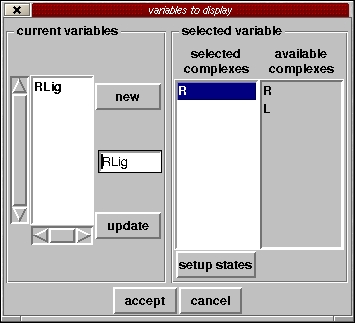
\includegraphics{vardispl.jpg}}} A new window, entitled
\emph{variables to display}, appears, presenting the current variables to
display. You can create a new variable or select existing ones. The maximal
number of variables you can display is \MAXNUMDISPLAYVARIABLES. To delete a
variable, select it and click while pressing the <Ctrl> key. Once a variable is
chosen, its name appears in the upper entry widget where you can change it.
The name of a variable to display is limited to \MAXOUTPUTVARNAMELENGTH{} characters.
As for several other entry widgets throughout the interface, the changes
of the name are recorded when the mouse quit the widget area, when you press
<Return> (\emph{not} the numeric pad <Enter>) or when another widget is focussed
(for instance with a <tab> press). The composition of the variable appears in
the middle-list. A variable can represent several complexes. You can add
complexes to the selected variable by drag and dropping them from the right
list. A variable can contain up to \MAXTYPESINOUTPUTVAR{} complexes. To delete a
complex from a variable, select it and click while pressing the <Ctrl> key. A
variable can represent specific states of a multistate complex. In such a case,
the variable can include only one complex type. To configure the states to be
displayed, select the complex and click on the button ``setup states''. If you
add another complex to a variable already containing a multistate complex, this
multistate is then considered as a regular complex and the variable is supposed
to display all its states. Therefore you cannot configure the states anymore.
This possibility reappears if you delete all the other complexes but the
multistate from the variable.

\parpic{\scalebox{0.4}{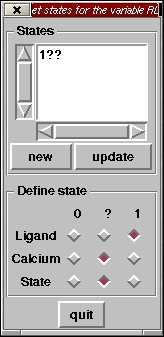
\includegraphics{displstates.jpg}}} When you decide to
choose which states of a multistate complex you want to
display\footnote{Remember, this is possible only if the variable contains only
  this multistate.}, a new window pops-up, entitled \emph{variable NAME}. A state
is defined by a certain configuration of all the flags (`set' or `1', `unset'
or `0' and `undefined' or `?').  You can create a new state with the ``new''
button (all the flags are initially at `?').  The various flags of the
multistate complex can be configured with the radiobuttons. As usual, after
having selected a state, you can click while pressing the <Ctrl> key to delete
it.

Once all your variables are set, you can record the changes you made and close
the \emph{variables to display} window by clicking the ``accept'' button. The
``cancel'' button will close the window without changing your configuration.

When you close the \emph{General configuration} window, the changes are
recorded. Be careful to undo all the changes you made if you want to ignore
them. Indeed there is currently no ``cancel'' button.

\subsection{Creating elementary components of the simulation}

The elementary building blocks of the simulation are the components, which
permit to make up the complexes, i.e. the actually reacting entities.  You can
select an existing component with the browsing list, or click on the nearby
``new'' button to create a new one. Up to \MAXCOMPONENTS{} components can be
created per simulation.

\parpic{\scalebox{0.4}{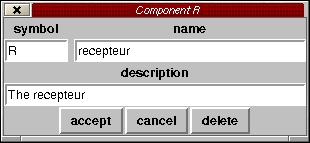
\includegraphics{component.jpg}}} A \emph{Component
  [SYMBOL]} window pops-up, allowing the configuration of the component
\emph{SYMBOL}.  In this window, you can enter a symbol for the component, a
name, and a description. The symbol is important since it will be used to
construct the name of the complexes including this component (maximal length
\MAXCOMPONENTSYMBOLLENGTH{} characters). Note that symbols can overlap but
cannot be included one into another. For instance, symbols AB and AC can
coexists, but not symbols A and AB. This insure the unequivocal decomposition of
the symbol of a complex into its components (see section \ref{make_complexes}).
The name can be longer and more explicit (maximal length
\MAXCOMPONENTNAMELENGTH{} characters). For instance the symbol can be `p' and
the name ``phosphate''.

Clicking the three lowest buttons will close the \emph{Component [SYMBOL]}
window, either recording the changes, cancelling them or totally removing the
component. A component cannot be removed if it is part of a complex.

\subsection{Creating complexes involved in the simulation}\label{make_complexes}

The complexes are the actual reacting entities of the simulation. You can select
an existing complex with the browsing list, or click on the nearby ``new''
button to create a new one. Up to \MAXCOMPLEXTYPES{} different complexes can be
created per simulation.

\parpic{\scalebox{0.5}{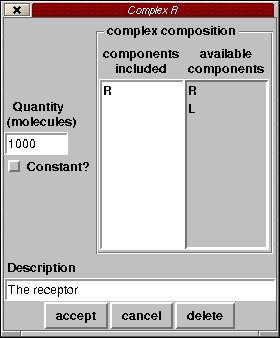
\includegraphics{complex.jpg}}} A \emph{Complex [SYMBOL]}
window pops-up, allowing the configuration of the complex \emph{SYMBOL}. To add
a component to the current complex, drag it from the rightmost list to the left
one. To remove a component from the current complex, select it from the leftmost
list and click while pressing the <Ctrl> key. \emph{The order of the components
  is important. A complex made of A then B is different from a complex made of B
  then A}. This allows the definition of complexes which include several times
the same component, but in different places or the definition of complexes made
up of the same components in different order. Up to \MAXCOMPONENTSINCOMPLEX{}
components can be part of a complex.  In the left entry widget, enter the
initial quantity of this complex, at the beginning of the simulation.  Note that
this must be expressed in number of molecules, not in concentration. If you
check the tickbox ``Constant?'', the concentration of that complex will be
maintained constant throughout the simulation\footnote{In order to do that, the
  GUI tranforms all the bimolecular reactions into unimolecular reactions,
  merging the rate constants and the concentrations of the constant substrates.
  In the Lotka-Voltera example provided with the distribution, compare for
  instance the values of the kf rate constant for the reaction
  $X+Y_1\rightarrow2Y_1$ shown in the GUI and in the file
  \texttt{REACTION.INI}.}. Be careful not to fix the concentration of a complex
involved in unimolecular reactions, or to fix the concentration of a multistate
complex.

Clicking the three lowest buttons will close the \emph{Complex [SYMBOL]}
window, either recording the changes, cancelling them or totally removing the
complex. A complex cannot be removed if it is part of a reaction or if a
multistate complex is based on it.

\newpage

\subsection{Creating multistate complexes}\label{make_multistates}

The multistate complexes are a special kind of reacting entities which possess
several binary flags describing their various possible states (see section
\ref{intro_multistates}).  You can select an existing multistate complex with
the browsing list, or click on the nearby ``new'' button to create a new one.

\parpic{\scalebox{0.5}{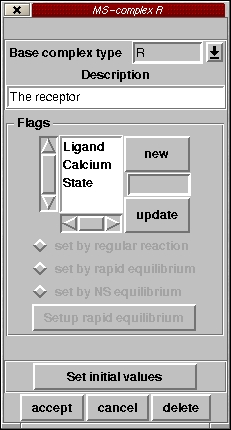
\includegraphics{multistate.jpg}}} A \emph{MS-complex
  [SYMBOL]} window pops-up, allowing the configuration of the multistate complex
\emph{SYMBOL}.  Each multistate complex has to be based on one of the complexes
previously defined (see section \ref{make_complexes}). If a complex is already
defined as multistate, you cannot use it for another multistate configuration
(create another complex instead). You can change the complex a multistate is
based on. If you do that \emph{the previous multistate configuration will be
  deleted}. This feature cannot currently be used to duplicate multistate
configuration between complexes.

You can create new flags (``new'' button). The name of a flag cannot have more than
\MAXMSFLAGLENGTH{} characters. To remove a flag from the complex, select it
and click while pressing the <Ctrl> key. Up to \MAXMSNUMFLAGS{} can be created
for each multistatee  complex.

The state of each flag can be controlled either by a standard reaction (see
section \ref{reactions}), or by a rapid equilibrium (see section \ref{ms_ini})
(if you are using the spatial extensions, there are actually two different kinds
of rapid equilibria, see section \ref{neighboursensitive}). You can change the
mode of control of each flag.  However, be careful and take a break before to do
so. Indeed, a quite complex configuration of a rapid equilibrium can be easily
wiped-out if you decide to reverse to a control by a ``regular'' reaction. In
order to change the control mode from ``reactions'' to ``rapid equilibrium'',
all the reactions involved have to be suppressed before.

If a flag has to be controlled by a classical multistate rapid equilibrium, you
have to setup the probability that it is ON, depending on the state of the
entire complex. To do so, press on the button ``Setup rapid equilibrium''.

\parpic{\scalebox{0.5}{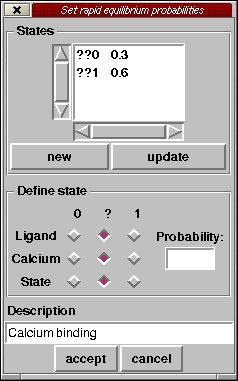
\includegraphics{MSrap_equil.jpg}}} A window \emph{set
  rapid equilibria properties} pops-up. You can create new states with the
``new'' button, and specifies the configuration of each flag with the
radiobuttons.  After selecting a state, you can click while pressing the <Ctrl>
key to delete it. The probability to set the controlled flag, depending on the
state of all the other flags, can be entered in the right entry widget.If you
add a flag later on, its value will be set at `?' in all the rapid-equilibria
and reaction states\footnote{This is also true for all the variables to display
  and the array snapshots by the way.}.

A rapid equilibrium can be controlled by a dynamic value (see section
\ref{dynamic_ini}). In such a case, the value you enter here has to be the
highest probability for the flag to set. This value will be replaced by the
adequat dynamic value when the event timepoints will arrive.

Once your probabilities are set, you can record the changes you made and close
the \emph{rapid equilibrium} window by clicking the ``accept'' button. The
``cancel'' button will close the window without changing your configuration.

Once all the flags are defined, the initial quantity of the complex in the
various states at the beginning of the simulation can be setup.

\parpic{\scalebox{0.5}{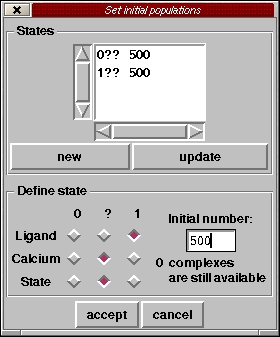
\includegraphics{ms_states.jpg}}} A click on the button
``Set initial values'' will cause a new window to pops-up, entitled \emph{Set
  initial populations}.  Several states can be defined by setting up the various
flags of the multistate complex. You can create new states with the ``new''
button.  For each particular state, you can specify the number of complexes in
this state at the beginning of the simulation. The sum of all states cannot be
superior to the total initial number of the current complex, defined previously
(see \ref{make_complexes}).  As usual after selecting a state you can click
while pressing the <Ctrl> key to delete it.

Once all the desired initial values are set, you can commit the changes and
quit (``accept'' button) or quit without recording changes (``cancel'' button).

Clicking the three lowest buttons of the \emph{MS-complex [SYMBOL]} window will
close it, either recording the changes, cancelling them or totally removing the
multistate configuration of the complex. Note that a multistate configuration
cannot be suppressed if a neighbour-sensitive complex is based on that
multistate complex.

\subsection{Creating neighbour-sensitive complexes}\label{neighboursensitive}

The neighbour-sensitive complexes are a special kind of multistate complexes
which can react according to the state of their nearest neighbours. They will
form the elements of bidimentional lattice you will setup later on (see section
\ref{arrays}). You can select an existing neighbour-sensitive with the browsing
list, or click on the nearby ``new'' button to create a new one.

\parpic{\scalebox{0.5}{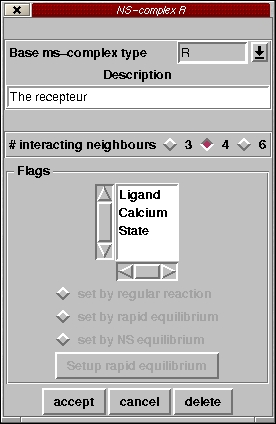
\includegraphics{neighboursensitive.jpg}}} A
\emph{NS-complex [SYMBOL]} window pops-up, allowing the configuration of the
neighbour-sensitive complex \emph{SYMBOL}.  Each neighbour-sensitive complex has
to be based on one of the multistate complexes previously defined (see section
\ref{make_multistates}). If a multistate complex is already defined as
neighbour-sensitive, you cannot use it for another neighbour-sensitive
configuration (create another complex instead). You can change the multistate
complex a neighbour-sensitive is based on. If you do that \emph{the previous
  neighbour-sensitive configuration will be deleted}. This feature cannot
currently be used to duplicate neighbour-sensitive configuration between
complexes.

The state of each flag can be controlled either by a standard reaction (see the
section \ref{reactions}), or by a rapid equilibrium (see section \ref{ms_ini}).
If you are using the spatial extensions, there are actually two different kinds
of rapid equilibria \footnote{You would not read that part if you aren't, or
  would you?}. You can change the mode of control of each flag.  However, be
careful and take a break before to do so. Indeed, a quite complex configuration
of a rapid equilibrium can be easily wiped-out if you decide to reverse to a
control by a ``regular'' reaction.  In order to change the control mode from
``reactions'' to ``NS rapid equilibrium'', all the reactions involved have to be
suppressed before.

If a flag has to be controled by a neighbour-sensitive rapid equilibrium press
on the button ``Setup rapid equilibrium''.

\parpic{\scalebox{0.5}{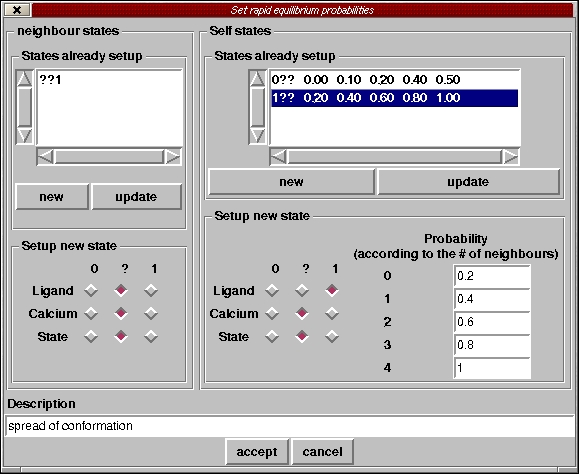
\includegraphics{NSrap_equil.jpg}}} A window \emph{set
  rapid equilibria properties} pops-up. You have to setup the probabilities that
it is ON, depending on the state of the entire complex (rightmost frame),
\emph{as well as the states of its nearest-neighbours} (leftmost frame). To do
so, If a complex has N neighbours (N depending on the geometry of the lattice
containing this neighbour-sensitive complex), N+1 probabilities have to be set
for each defined state, corresponding to 0,1 \ldots N neighbours being in the
particular states defined in the leftmost frame.

In both frames you can create new states with the ``new'' button, and specifies
the configuration of each flag with the radiobuttons. After selecting a state,
you can click while pressing the <Ctrl> key to delete it. The probabilities to
set the controled flag, depending on the state of the other flags, can be
entered in the right entry widgets.

Once your probabilities are set, you can record the changes you made and close
the \emph{rapid equilibrium} window by clicking the ``accept'' button. The
``cancel'' button will close the window without changing your configuration.

Clicking the three lowest buttons of the \emph{NS-complex [SYMBOL]} window will
close it, either recording the changes, cancelling them or totally removing the
neighbour-sensitive configuration of the complex.

\subsection{Configuration of the bidimensional lattice}\label{arrays}

In order to react with their neighbours, the neighbour-sensitive complexes have
to be arranged into bidimensional lattice, or arrays. A simulation can contain
several arrays. You can select an existing array with the browsing list, or
click on the nearby ``new'' button to create a new one. Up to 
\MAXNUMCOMPLEXARRAYS{} arrays can be created by simulation.

\parpic{\scalebox{0.5}{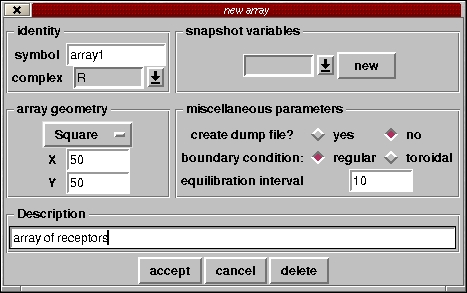
\includegraphics{array.jpg}}} A window \emph{Array
  [SYMBOL]} pops-up, allowing the configuration of the array \emph{SYMBOL}.  See
the section \ref{array_ini} for more details about the various options.  In the
frame ``Identity'', you can chose a symbol for the array (maximum
\MAXARRAYNAMELENGTH{} characters) and select the neighbour-sensitive complex it
will be made of.  The current version of \stochsim{} use only homogenous arrays,
made of one type of complex only.

The
frame ``Array geometry'' permits to setup the size of the array, but also its
topology, i.e. the number of neighbours each complex can react with. The maximal
allowed width is \MAXARRAYWIDTH{} and the maximal allowed length is
\MAXARRAYLENGTH{}.

If the ``boundary condition'' is set to ``regular'', a complex located on the
edge of the array will have less neighbours than the others. On the contrary,
if the the ``boundary condition'' is set to ``toroidal'', the opposite edges
are connected, giving the array the topologie of a doughnut. In this
configuration, all complexes have the same number of complexes.  The
``equilibration interval'' value controls the frequency of the re-equilibration
of all the flags controlled by a neighbour-sensitive rapid equilibrium.

The snapshot-variables are the spatial equivalent of the variable to display.
They represent selected states of each complex in the array. You can select an
existing snapshot-variables with the browsing list, or create a new one by
clicking on the nearby ``new'' button. Up to \MAXNUMARRAYSNAPSVARIABLES{}
snapshot variables can be defined for each array.

\parpic{\scalebox{0.5}{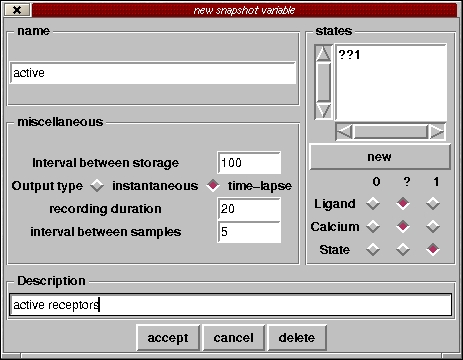
\includegraphics{snaps.jpg}}} A window \emph{Snapshot
  variable [NAME]} pops-up, allowing to configure the snapshot-variable
\emph{NAME}. The name of a snapshot variables is limited to
\MAXARRAYVARNAMELENGTH{} characters.

The frame ``Output characteristics'' allows the configuration of the frequency
and the type of data storage. The ``interval between storage'' specifies the
interval between two storages of the states of the array. Tthe states are
defined in the rightmost frame ``States''. Up to \MAXNUMARRAYSNAPSSTATES{}
states can be represented by each snapshot variable.  If the ``output type'' is
``instantaneous'', the current states of the array is stored. If the ``output
type'' is ``time-lapse'', an average of the states will be stored. The states
will be averaged according the value of ``recording duration'' (which has to be
lower than the ``interval between storage''). The number of averaged snapshot is
deciphered by the value ``interval between samples''(if it is equal to
``recording duration'', only one snapshot is recorded, rendered the output
equivalent to an instantaneous one).

Clicking the three lowest buttons of the \emph{Array [SYMBOL]} window will close it,
either recording the changes, cancelling them or totally removing the array.

\subsection{Creating reactions}\label{reactions}
The reactions are the ``standard'' way for the molecules to interact in the
simulation.  You can select an existing reaction with the browsing list, or
create a new one by clicking on the nearby ``new'' button.

\parpic{\scalebox{0.4}{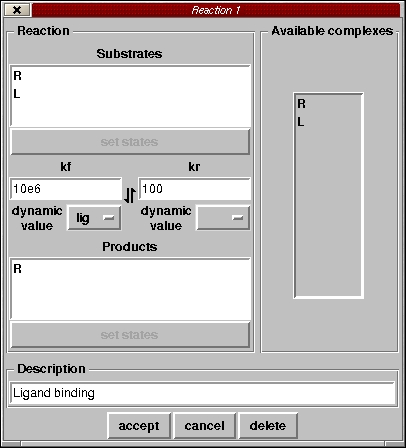
\includegraphics{reaction.jpg}}} A \emph{Reaction X} window
pops-up, allowing the configuration of the reaction \emph{X}. To add a complex as a
substrate or a product, select it in the list on the right, and drag it either in
the substrate list or the product list.  To remove a complex from either the
substrates or the products, select it from the appropriate list and click while
pressing the <Ctrl> key. Note that a reaction has to contain at least one
non-constant substrate and one non-constant product.

Enter the forward and reverse rate in units of s\textsuperscript{-1} or
M\textsuperscript{-1}$\cdot$s\textsuperscript{-1} (according to the order of the
reaction). If a substrate or a product is a multistate complex, you can further
refined the effect of the reaction on the complex, and the effect of the states
on the rate constants.

\vspace{2.5\baselineskip}

\parpic{\scalebox{0.4}{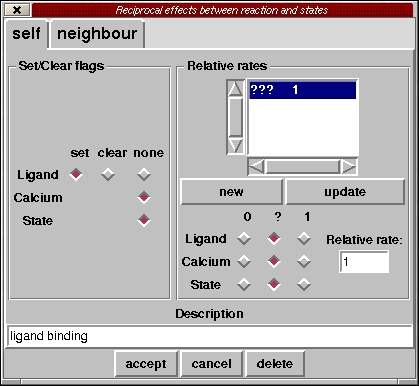
\includegraphics{MSreaction.jpg}}} A click on the button
``set states'' (activated when you select a multistate complex) will pops-up a
new window. Two tabs are present ``self'' and ``neighbour''. The second tab is
activated only when the spatial extensions are used. 

The ``self'' tab permits to configure the classical involvement of a multistate
complex in a reaction.  The left frame permits to set-up the effect of the
reaction on the complex, i.e. to set or clear particular flags. A flag which is
set up by a rapid equilibrium (either multistate or neighbour-sensitive) cannot
be modified here. Change its status first, as explained in the section
\ref{make_multistates}.  The right frame permits to define several states (i.e.
sets of flag values) and their effects on the basal reaction rate.  

\parpic{\scalebox{0.4}{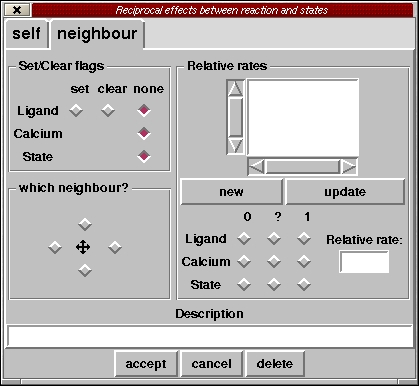
\includegraphics{NSreaction.jpg}}} The ``neighbour'' tab
permits to configure the effect of a neighbour-sensitive complex on the reaction
involving one of its neighbours. The left-top frame permits to set-up the effect
of the reaction on the neighbouring complex, i.e. to set or clear particular
flags. A flag which is set up by a rapid equilibrium (either multistate or
neighbour-sensitive) cannot be modified here. Change its status first, as
explained in the section \ref{make_multistates}.  The right frame permits to
define several states (i.e.  sets of flag values) of the complex and their
effects on the basal rate of the reaction that its neighbour undergoes. Finally
the left-bottom frame allow to choose which neighbour is affected. The number of
possible neighbours depends on the geometry of the lattice containing these
neighbour-sensitive complexes.

Once all the desired values are set, you can commit the changes and quit
(``accept'' button) or quit without recording changes (``cancel'' button).
 
Clicking the three lowest buttons will close the \emph{Reaction} window, either
recording the changes, cancelling them or totally removing the reaction.

\section{Setting-up the dynamic values}

\section{Running a simulation}

Once setup, the simulation can be launched from Tk\stochsim{} by choosing using
``run'' from the ``simulation'' menu, or by typing \mbox{<ctrl-r>}. \emph{Be
  careful, as the configuration is automatically saved before the simulation is
  run}. You can kill this simulation with the item ``stop'' of the ``simulation'' menu.
Note that once \stochsim{} is launched, it is independent of the Tk interface.
When quitting, Tk\stochsim{} \emph{will not kill} \stochsim{}.  When a
simulation has been launched you can load, modify and save other simulations.
You can also visualise the results recorded previously. However you cannot
run another simulation. To do so, launch another instance of the interface.

To quit Tk\stochsim{}, use the menu ``File->Quit'', click the ``quit'' button or
type \mbox{<Ctrl-q>}.

\newpage

\section{Visualisation of the results}\label{display}

You can visualise the result of a simulation, stored in the file
\texttt{VAR.OUT}. To do so, click on the button ``view data'' and a text window
will pops-up. The same result can be achieved with the accelerator <Ctrl-v>.

\scalebox{0.4}{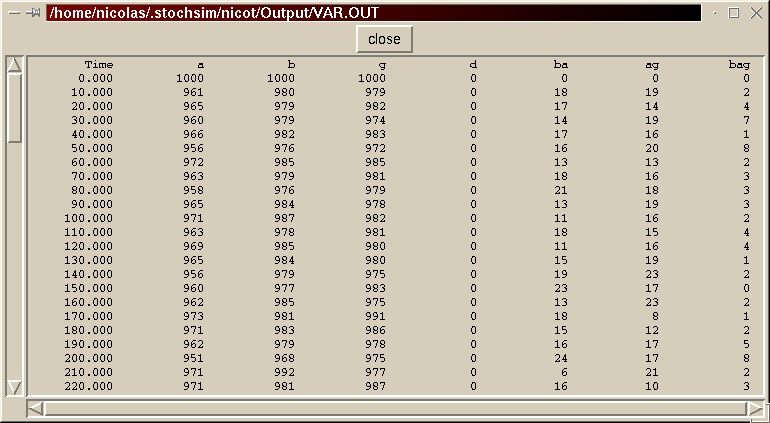
\includegraphics{viewdata.jpg}}

If the button ``show data'' is disabled, either no simulation are loaded, either
the file \texttt{VAR.OUT} does not exist (i.e. the simulation was never run).
Note that you can visualise the results while the simulation is running since
\stochsim{} periodically update the file \texttt{VAR.OUT}.

\parpic{\scalebox{0.4}{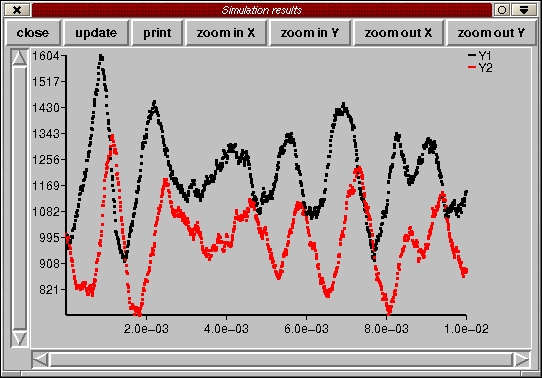
\includegraphics{plot.jpg}}} The results can also be
visualised graphically by clicking the button ``plot''. A graph window will then
pops-up, showing the time course of the variables you chose to display, or of
all the complexes, see section \ref{genconfig}. The same result can be achieved
with the accelerator <Ctrl-p>. The graphs will not automatically refresh.
However you can update them by clicking on the relevant button. The parameters
of the plot can be setup by editing the file \texttt{stochsimrc} directly or via
the menu ``Options>>Preferences''. After choosing a different background color
of plot size, you have to quit and relaunch the plotting window. However the
curves' colors and the type of plot is refreshed with each update. You can
zoom-in and zoom-out the graph, independently for both axis. Choose the
invariant point of the homothetic scaling with <Ctrl-Button1>. You can record
snapshots of the graph at any time, by saving it in a postscript file.

You can monitor the progress of the simulation with a progress bar
launched by the button ``monitor''. The progress bar will refresh itself
automatically. However this consumes memory and cpu time. Therefore it is better
to launch it periodically to probe the simulation progress but to kill it
otherwise.

%%% Local Variables: 
%%% mode: latex
%%% TeX-master: "stochsim_manual"
%%% End: 
